% -----------------------------------------------
% Template for ISMIR Papers
% 2016 version, based on previous ISMIR templates

% Requirements :
% * 6+1 page length maximum
% * 2MB maximum file size
% * Copyright note must appear in the bottom left corner of first page
% (see conference website for additional details)
% -----------------------------------------------

\documentclass{article}
\usepackage{ismir,amsmath,cite}
\usepackage{graphicx}
\usepackage{dsfont}
\usepackage{url}
\usepackage{color}

\usepackage{amsfonts}
\usepackage{stmaryrd}
\usepackage{xspace}
\usepackage{IEEEtrantools}
\newcommand*{\eg}{e.g.\@\xspace}
\newcommand*{\ie}{i.e.\@\xspace}

% Title.
% ------
\title{Wavelet Scattering for Automatic Chord Estimation}

% Note: Please do NOT use \thanks or a \footnote in any of the author markup

% Single address
% To use with only one author or several with the same address
% ---------------
%\oneauthor
% {Names should be omitted for double-blind reviewing}
% {Affiliations should be omitted for double-blind reviewing}

% Two addresses
% --------------
%\twoauthors
%  {First author} {School \\ Department}
%  {Second author} {Company \\ Address}

%% To make customize author list in Creative Common license, uncomment and customize the next line
%  \def\authorname{First Author, Second Author} 


% Three addresses
% --------------
\threeauthors
 {Chris Miller} {MARL, New York University \\ {\tt crm313@nyu.edu}}
  {Second Author} {\bf Retain these fake authors in\\\bf submission to preserve the formatting}
  {Third Author} {Affiliation3 \\ {\tt author3@ismir.edu}}

%% To make customize author list in Creative Common license, uncomment and customize the next line
%  \def\authorname{First Author, Second Author, Third Author} 

% Four or more addresses
% OR alternative format for large number of co-authors
% ------------
%\multauthor
%{First author$^1$ \hspace{1cm} Second author$^1$ \hspace{1cm} Third author$^2$} { \bfseries{Fourth author$^3$ \hspace{1cm} Fifth author$^2$ \hspace{1cm} Sixth author$^1$}\\
%  $^1$ Department of Computer Science, University , Country\\
%$^2$ International Laboratories, City, Country\\
%$^3$  Company, Address\\
%{\tt\small CorrespondenceAuthor@ismir.edu, PossibleOtherAuthor@ismir.edu}
%}
%\def\authorname{First author, Second author, Third author, Fourth author, Fifth author, Sixth author}


\sloppy % please retain sloppy command for improved formatting

\begin{document}

%
\maketitle
%
\begin{abstract}
The abstract should be placed at the top left column and should contain about 150-200 words.
\end{abstract}

%%%%%%%%%%%%%%%%%%%%%%%%%%%%%%%%%%%%%%%%%%%%%%%%%%

\section{Introduction}\label{sec:introduction}

Much work has been done in the domain of Automatic Chord Estimation (ACE) -- one of the so-called ``holy grails" of Music Information Retrieval (MIR) research. In general, ACE systems seek to analyze a particular audio file and generate a vector indicating the predominant chord in the song over a particular time frame (``C minor from 1.5 seconds to 4 seconds", for example). 
	
	Chord estimation systems developed at NYU's Music and Audio Research Lab (such as those detailed in \cite{cho2014on} \cite{humphrey2015four}) use supervised learning approaches to train a chord model on a large chord vocabulary of 157 different chords. Typically, these systems consist of three-part pipeline:
	\begin{description}
	\item{\textbf{Feature Extraction}} to transform the audio file into a musically relevant representation
	\item{\textbf{Pattern Matching}} to match the harmonic content in a particular time frame with a template in a trained chord model
	\item{\textbf{Decoding}} to determine whether or not a predicted chord makes sense in context
	\end{description}
	
	\textbf{Feature extraction} in the ACE systems of \cite{cho2014on} \cite{chothesis} uses a Constant-Q transform to create a frequency-space representation on a perceptual log-scale of ten octaves. That is, a pitch representation $\rho_{t,\lambda}$ encodes the energy in temporal window $t$ at a frequency band centered around $\lambda$, where each $\lambda$ corresponds to a pitch in traditional Western twelve-tone music theory. A $K$-multi-band chroma representation is then created by first windowing the frequency scale with $K$ Gaussians distributed evenly over the support of $\lambda$, and then by wrapping each windowed representation $\boldsymbol{X}[t,\gamma]$ into a chroma vector. This creates a new representation $\boldsymbol{Y}[t,q,k]$ which is invariant to octave transpositions where $q$ is an integer $\in [1,12]$ representing a chroma (or pitch) value, and $K$ is the windowed band. 
	
	\textbf{Pattern matching} is done by creating a chord model for all 157 chords with Gaussian Mixture Models (GMMs). This is a supervised learning approach where features are extracted for a large training set that contains examples of all 157 chords (with annotations) and are then used to train GMM templates for each chord. Data augmentation is employed by rotating each chord through the chroma space so that one example of C minor can also train a model for C\# minor, D minor, etc. For any temporal frame $t$, each of the $K$ chroma representations $\chi_{t,q}$ are matched using GMMs and then fused together via geometric mean. Finally, \textbf{decoding} uses Hidden Markov Model (HMM) systems to post-filter the pattern matched data. Here, we use the Viterbi algorithm, which describes the transition probability from one chord $C_i$ state to another -- $\mathds{P}(C_i \rightarrow C_j)$, therefore filtering out chord transitions that are highly unlikely. The matrix of transition probabilities for Viterbi decoding is generated from the labeled training data.
	
	Our experiments looked to replace parts of the existing feature extraction techniques with new ones based on Haar wavelet transforms and deep Haar scattering. We began with the MATLAB system designed by Taemin Cho available in \cite{choGithub} and added the new wavelet-based feature extraction routines to it.
	
%%%%%%%%%%%%%%%%%%%%%%%%%%%%%%%%%%%%%%%%%%%%%%%%%%

\section{Experimental Setup and Evaluation}\label{sec:experiment}
Evaluation of an ACE system was determined using some of the tools found in the \textsf{mir\_eval} library \cite{raffel2014mir} and written into a simple python script called \textsf{basic\_evaluate.py}, which compared the estimated chords coming out of the ACE system to the ground truth annotations for all songs in the testing set. All experiments were run on the High Performance Computing (HPC) environment at NYU's Courant Institute. 
	
For each experiment, the script \textsf{\textbf{extractFeaturesAndTrain}} is called first to both train a chord model and generate a Viterbi transition probability matrix. \textsf{extractFeaturesAndTrain} takes a list of training files (remaining constant throughout all experiments), as well as a directory to write the features, chord models, and transition matrices to. We adjusted this script to also take in a `mode' variable and a `band'. `mode' is a switch changing the feature extraction method between multiband chroma, Haar wavelet transforms, and deep Haar scattering. 'band' ($K$) determines the amount of chroma vectors at any given temporal window -- equivalent to the number of bands in the multiband chroma representation, and the maximum wavelet scale in the wavelet and scattering representations (i.e. the number of wavelet coefficients).
	
	Next, \textsf{\textbf{doChordID}} is called to perform the chord recognition task on the testing set. \textsf{doChordID} takes a list of test files (again, remaining constant throughout all experiments) as well as the directory containing the chord models and decoding matrices to use (i.e. the output of \textsf{extractFeaturesAndTrain}, and another directory to output the computed results. \textsf{doChordID} was also modified to take in a 'mode' switch -- the script automatically picks up the band $k$ from the GMM models in the trained chord models.
	
	Finally, \textsf{\textbf{basic\_evaluate.py}} is run over the test set to evaluate the results. As per \cite{raffel2014mir}, there is ``no single right way to compare two sequences of chord labels," and the \textsf{mir\_eval} package computes ACE accuracy based along metrics such as root, triads, maj/min, sevenths, inversions, etc. For simplicity, we evaluate all experiments using the \textsf{mirex} measure, which ``considers a chord correct if it shares at least three pitch classes in common" \cite{raffel2014mir}.
	
	State of the art systems such as those in \cite{cho2014on} use a multiband chroma feature extraction with $K = 4$ windowed bands. To begin, some baseline trials were run on a training set consisting of 111 songs from the Beatles discography, 99 RWC pop songs, 224 songs from the Billboard dataset, and 20 Queen songs, for a total of 454 songs. Our testing dataset comprised of 53 Beatles songs that were not part of the training set. Once again, these training and testing sets were kept constant across all experiments. For the $K = 4$ multiband system, the \textsf{MIREX} evaluation is \textbf{66.7\%}.
	
The constant-Q spectrogram $\boldsymbol{X}[t, \gamma]$ is reshaped into a time-chroma-octave
representation $\boldsymbol{X}[t, q, u]$ where the chroma index $q \in \llbracket 0 ; Q \llbracket$ and
octave index $u \in \llbracket 0 ; K \llbracket$ are derived from the log-frequency index $\gamma$
by Euclidean division: $\gamma = Q \times u + q$.
All subsequent operations apply to the octave variable $u$, and are vectorized in terms of time
$t$ and chroma $u$. To alleviate notations, we replace the three-way tensor $\boldsymbol{X}[t, q, u]$
by a vector $\boldsymbol{x}[u]$, thus leaving the indices $t$ and $q$ implicit.

%%%%%%%%%%%%%%%%%%%%%%%%%%%%%%%%%%%%%%%%%%%%%%%%%%

\section{Haar Wavelet Transform}\label{sec:haar}
Dating back to 1909, the Haar wavelet $\psi$ is a piecewise constant, real function of compact
support, consisting of two steps of equal length and opposite values. Within a discrete framework,
it is defined by the following formula:
\begin{equation}
\forall u \in \mathbb{Z}, \;
\boldsymbol{\psi}[u] = \left\{ \begin{array}{cl}
\frac{-1}{\sqrt{2}} & \mbox{if }u = 0\\
\frac{1}{\sqrt{2}} & \mbox{if }u = 1\\
0 & \mbox{otherwise}
\end{array}\right.
\end{equation}
The "mother" wavelet $\boldsymbol{\psi}[u]$ is translated and dilated by powers of two, so as to
produce a family of discrete sequences
$\boldsymbol{\psi_{j,b}}[u] = 2^{j/2} \boldsymbol{\psi}[2^j (u - 2b)]$
indexed by the scale parameter $j \in \mathbb{N}$ and the translation parameter $b \in \mathbb{Z}$.
After endowing them with the Euclidean inner product
\begin{equation}
\langle \boldsymbol{\psi_{j,b}} \vert \boldsymbol{\psi_{j^\prime,b^\prime}} \rangle
 =
 \sum_{u = -\infty}^{+\infty}
 \boldsymbol{\psi_{j, b}}[u]
  \boldsymbol{\psi_{j^\prime,b^\prime}}[u],
\end{equation}
the wavelets $\{\boldsymbol{\psi_{j,b}}\}_{j,b}$ form an orthonormal basis of finite-energy
real sequences.
Moreover, the Haar wavelet is the shortest function of compact support such that the family
$\{\boldsymbol{\psi_{j,b}}\}_{j,b}$ satisfies this orthonormality property.
On the flip side, it has a poor localization in the Fourier domain, owing to its sharp discontinuities.
Elements of the Haar wavelet basis are shown on Figure \ref{fig:haar-wavelets}
for various values of $j$ and $b$.

\begin{figure}[t]
    \begin{center}
        \setlength{\unitlength}{1cm}
        \begin{picture}(8.5,8.8)
        \put(0,-0.5){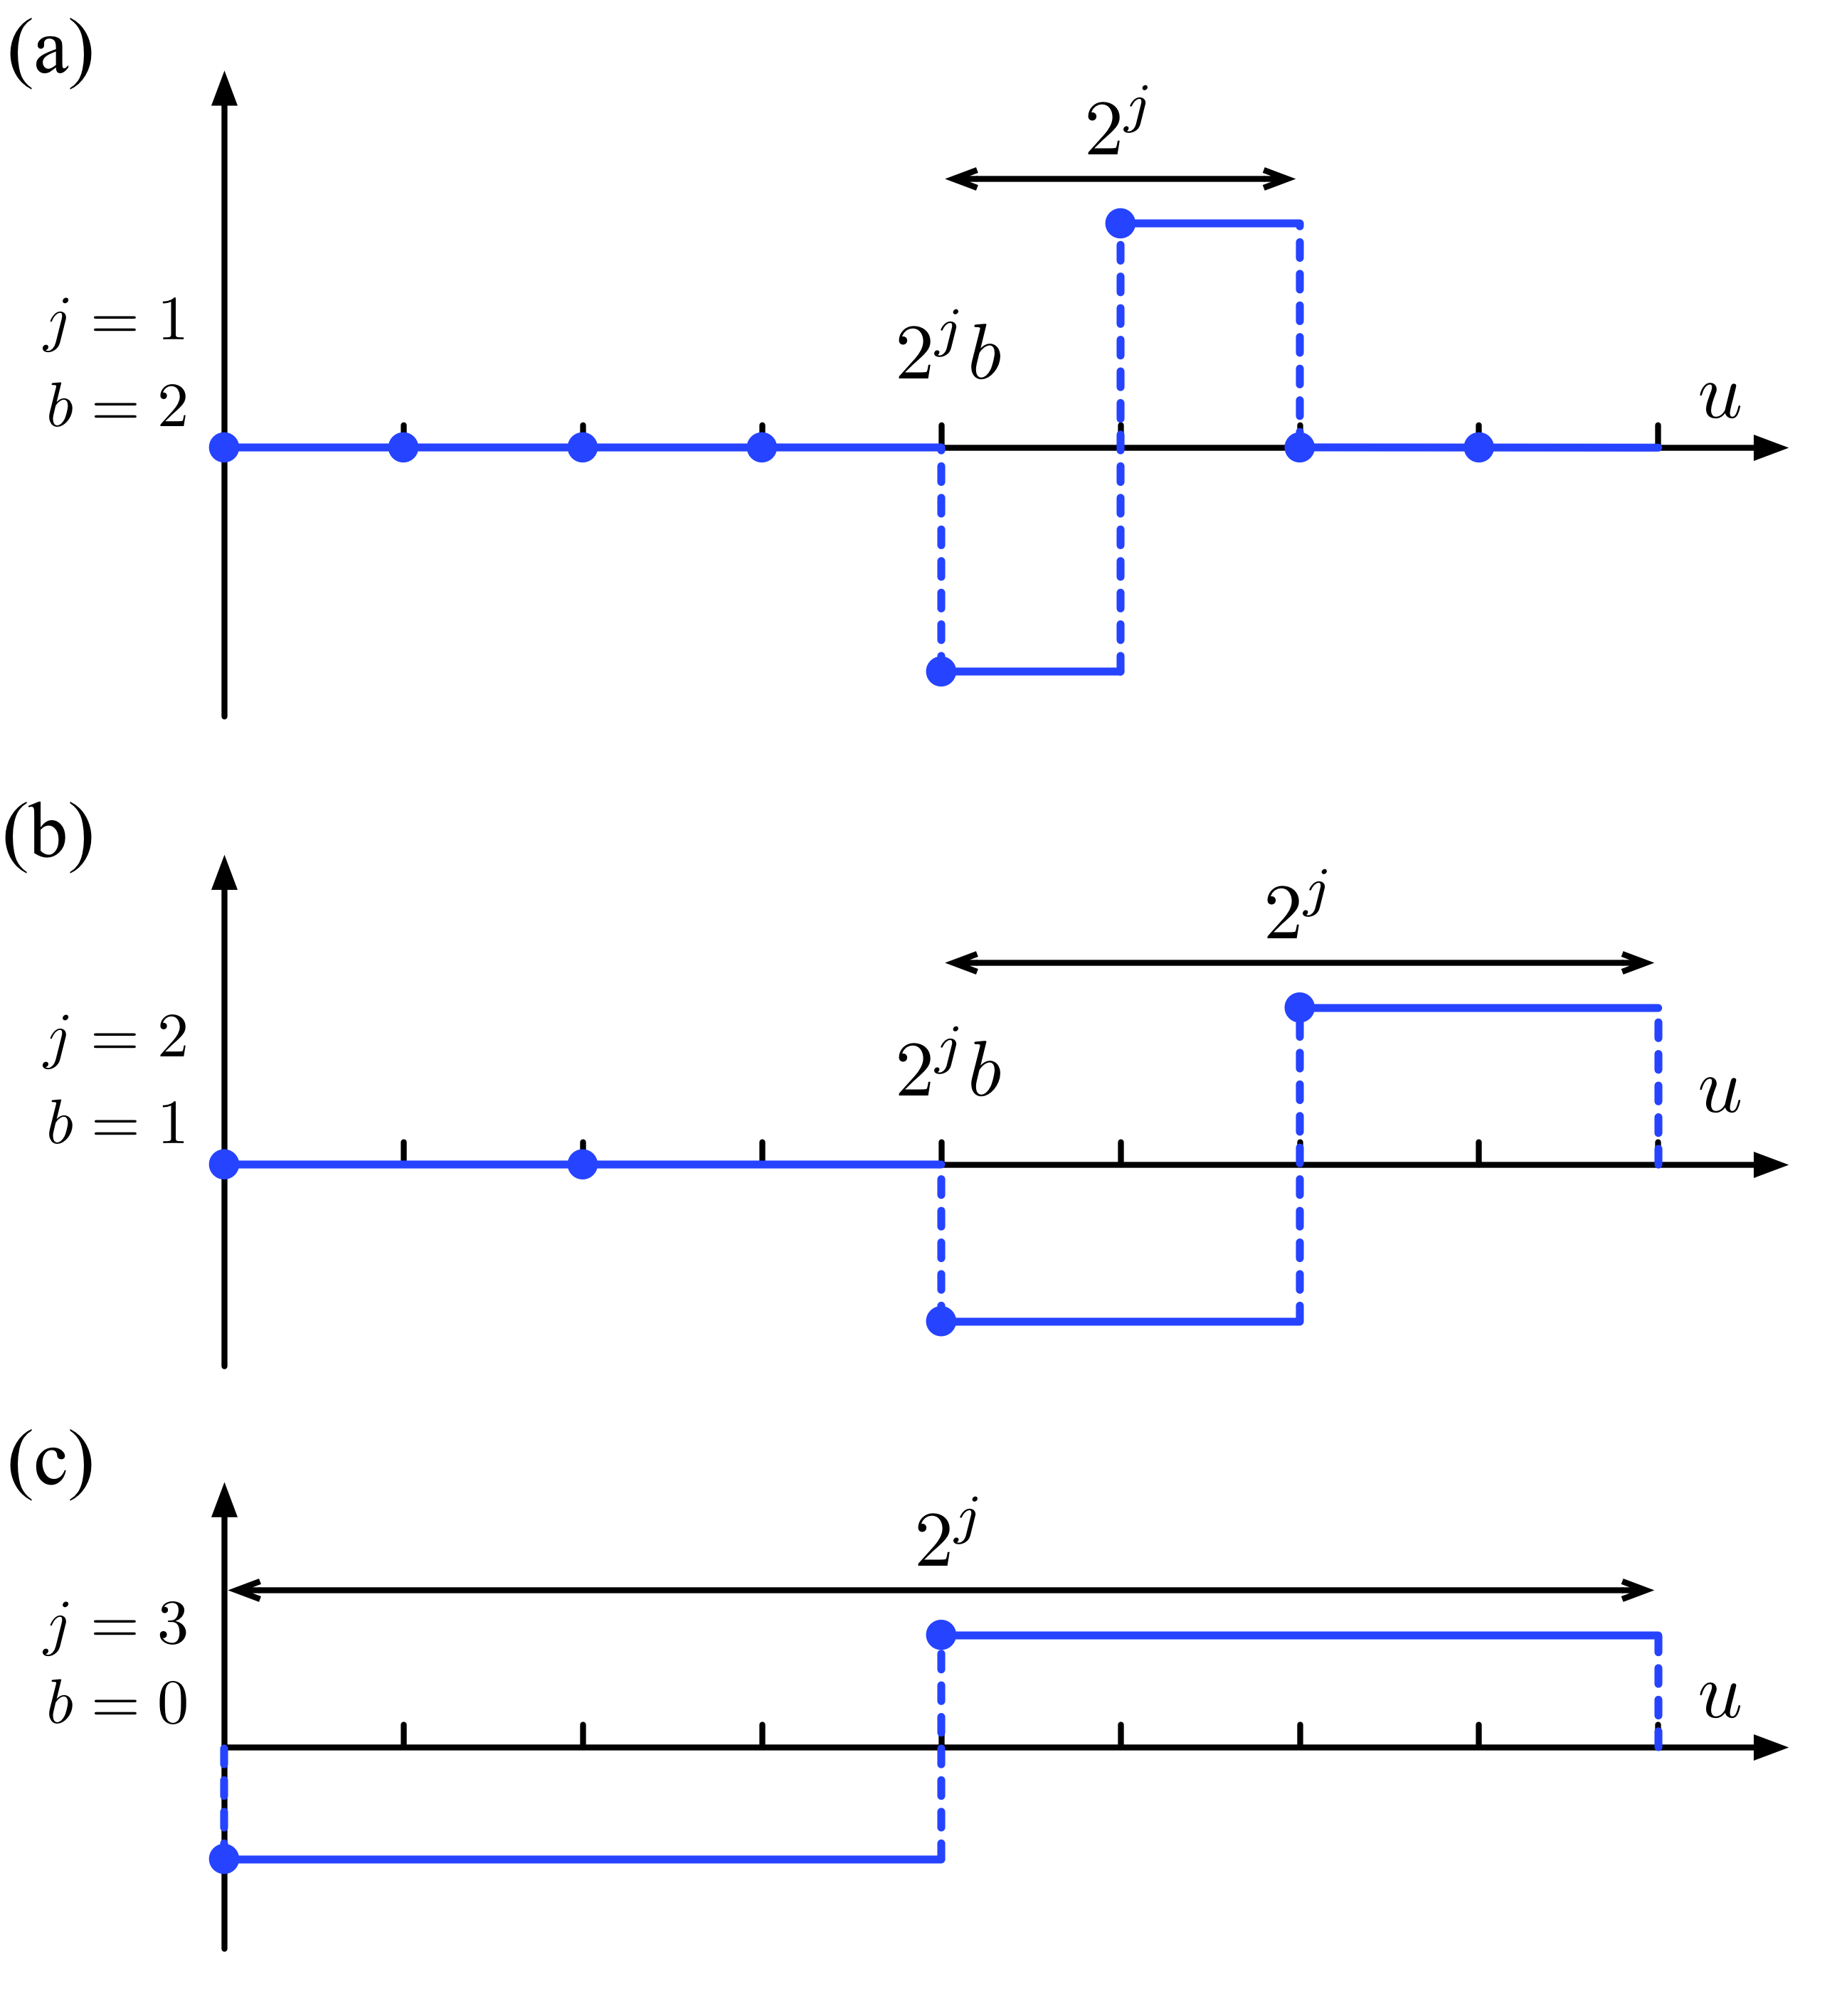
\includegraphics[width=8.5cm]{figs/haar_functions.png}}
        \end{picture}
    \end{center}
    \protect\caption{
Three elements of the Haar wavelet basis $\{ \boldsymbol{\psi_{j,b}}\}$
for various values of the scale index $j$ and the translation index $b$.
See text for details.
\label{fig:haar-wavelets}
}
\end{figure}

The wavelet transform coefficients of some finite-energy sequence
$\boldsymbol{x} \in \ell^2(\mathbb{Z})$ are defined by
$\boldsymbol{Wx}[j, b] = \langle \boldsymbol{x} \vert \boldsymbol{\psi_{j,b}} \rangle$.
Since $\boldsymbol{x}[u]$ has a finite length $K = 2^J$, the above decomposition is informative
only for indices $(j, b)$ such that $j < J$ and $2^j b < K$, that is $b<2^{J-j}$.
The number of coefficients in the Haar wavelet transform of $\boldsymbol{x}[u]$ is thus equal to
$\sum_{j<J} 2^{J-j} = 2^J - 1$. For the wavelet representation to
preserve energy and allow signal reconstruction, a residual term
\begin{equation}
\boldsymbol{A_J x}
= \boldsymbol{x}[0] -
\sum_{j,b}
\langle \boldsymbol{x} \vert \boldsymbol{\psi_{j,b}} \rangle \boldsymbol{\psi_{j,b}}[0]
= \sum_{u<K} \boldsymbol{x}[u]
\end{equation}
must be appended to the wavelet coefficients.
Observe that $\boldsymbol{A_J x}$ computes a delocalized average of all signal
coefficients, which can equivalently be formulated as an inner product with the constant
function $\boldsymbol{\phi}[u] = 2^{-J/2}$ over the support $\llbracket 0 ; K \llbracket$.
Henceforth, it corresponds to the traditional chroma representation, where spectrogram bands
of the same pitch class $q$ are summed across all $K$ octaves.

Since the wavelet representation amounts to $K$ inner products in $\mathbb{R}^K$,
its computational complexity is $\Theta(K^2)$ if implemented as a matrix-vector product.
Implementing these inner products as convolutions would bring the complexity to
$\Theta{(K (\log_2 K)^2)}$ by using the Fast Fourier Transform (FFT) algorithm.
To improve this, Mallat has developed a recursive scheme, called
\emph{multiresolution pyramid} \cite{mallat1989theory}, which operates as a cascade
of convolutions with some pair of quadrature mirror filters
$(\boldsymbol{g}, \boldsymbol{h})$ and progressive downsamplings by a factor of two.

\begin{equation}
\boldsymbol{Wx}[j,b] =
\left(
\boldsymbol{h_{\downarrow 2}} \circ
\boldsymbol{g_{\downarrow 2}} \circ \ldots \circ
\boldsymbol{g_{\downarrow 2}}\boldsymbol{x}
\right)[b]
\end{equation}

\begin{equation}
\boldsymbol{A_J x} =
\boldsymbol{g_{\downarrow 2}} \circ \ldots \circ
\boldsymbol{g_{\downarrow 2}}\boldsymbol{x}
\end{equation}

The associated Z-transforms $G$ and $H$ of $\boldsymbol{g}$
and $\boldsymbol{h}$ satisfy the quadrature mirror property $G(z) = H(-z)$ and
energy conservation: $\vert G(z) \vert ^2 + \vert H(z) \vert ^2 = 1$.
The interested reader can refer to chapter 7 of Mallat's textbook \cite{mallat2008wavelet},
of which we adopt the mathematical notations.

In the case of Haar wavelets, the low-pass filtering $(\boldsymbol{x} \ast \boldsymbol{g})$
consists of the sum between adjacent coefficients, whereas the high-pass filtering
$(\boldsymbol{x} \ast \boldsymbol{h})$ is the coresponding difference, up to a
renormalization constant:

\begin{equation}
(\boldsymbol{x}
\ast
\boldsymbol{g})[2b]
=
\frac{ \boldsymbol{x}[2b+1] + \boldsymbol{x}[2b]}{\sqrt{2}}
=
\boldsymbol{x}[2b]
-
\langle \boldsymbol{x} \vert \boldsymbol{\psi_{0,b}} \rangle
\end{equation}

\begin{equation}
(\boldsymbol{x}
\ast
\boldsymbol{h})[2b]
=
\frac{ \boldsymbol{x}[2b+1] - \boldsymbol{x}[2b]}{\sqrt{2}}
=
\langle \boldsymbol{x} \vert \boldsymbol{\psi_{0,b}} \rangle.
\end{equation}

\begin{figure}[t]
    \begin{center}
        \setlength{\unitlength}{1cm}
        \begin{picture}(8,2.5)
        \put(0,-0.5){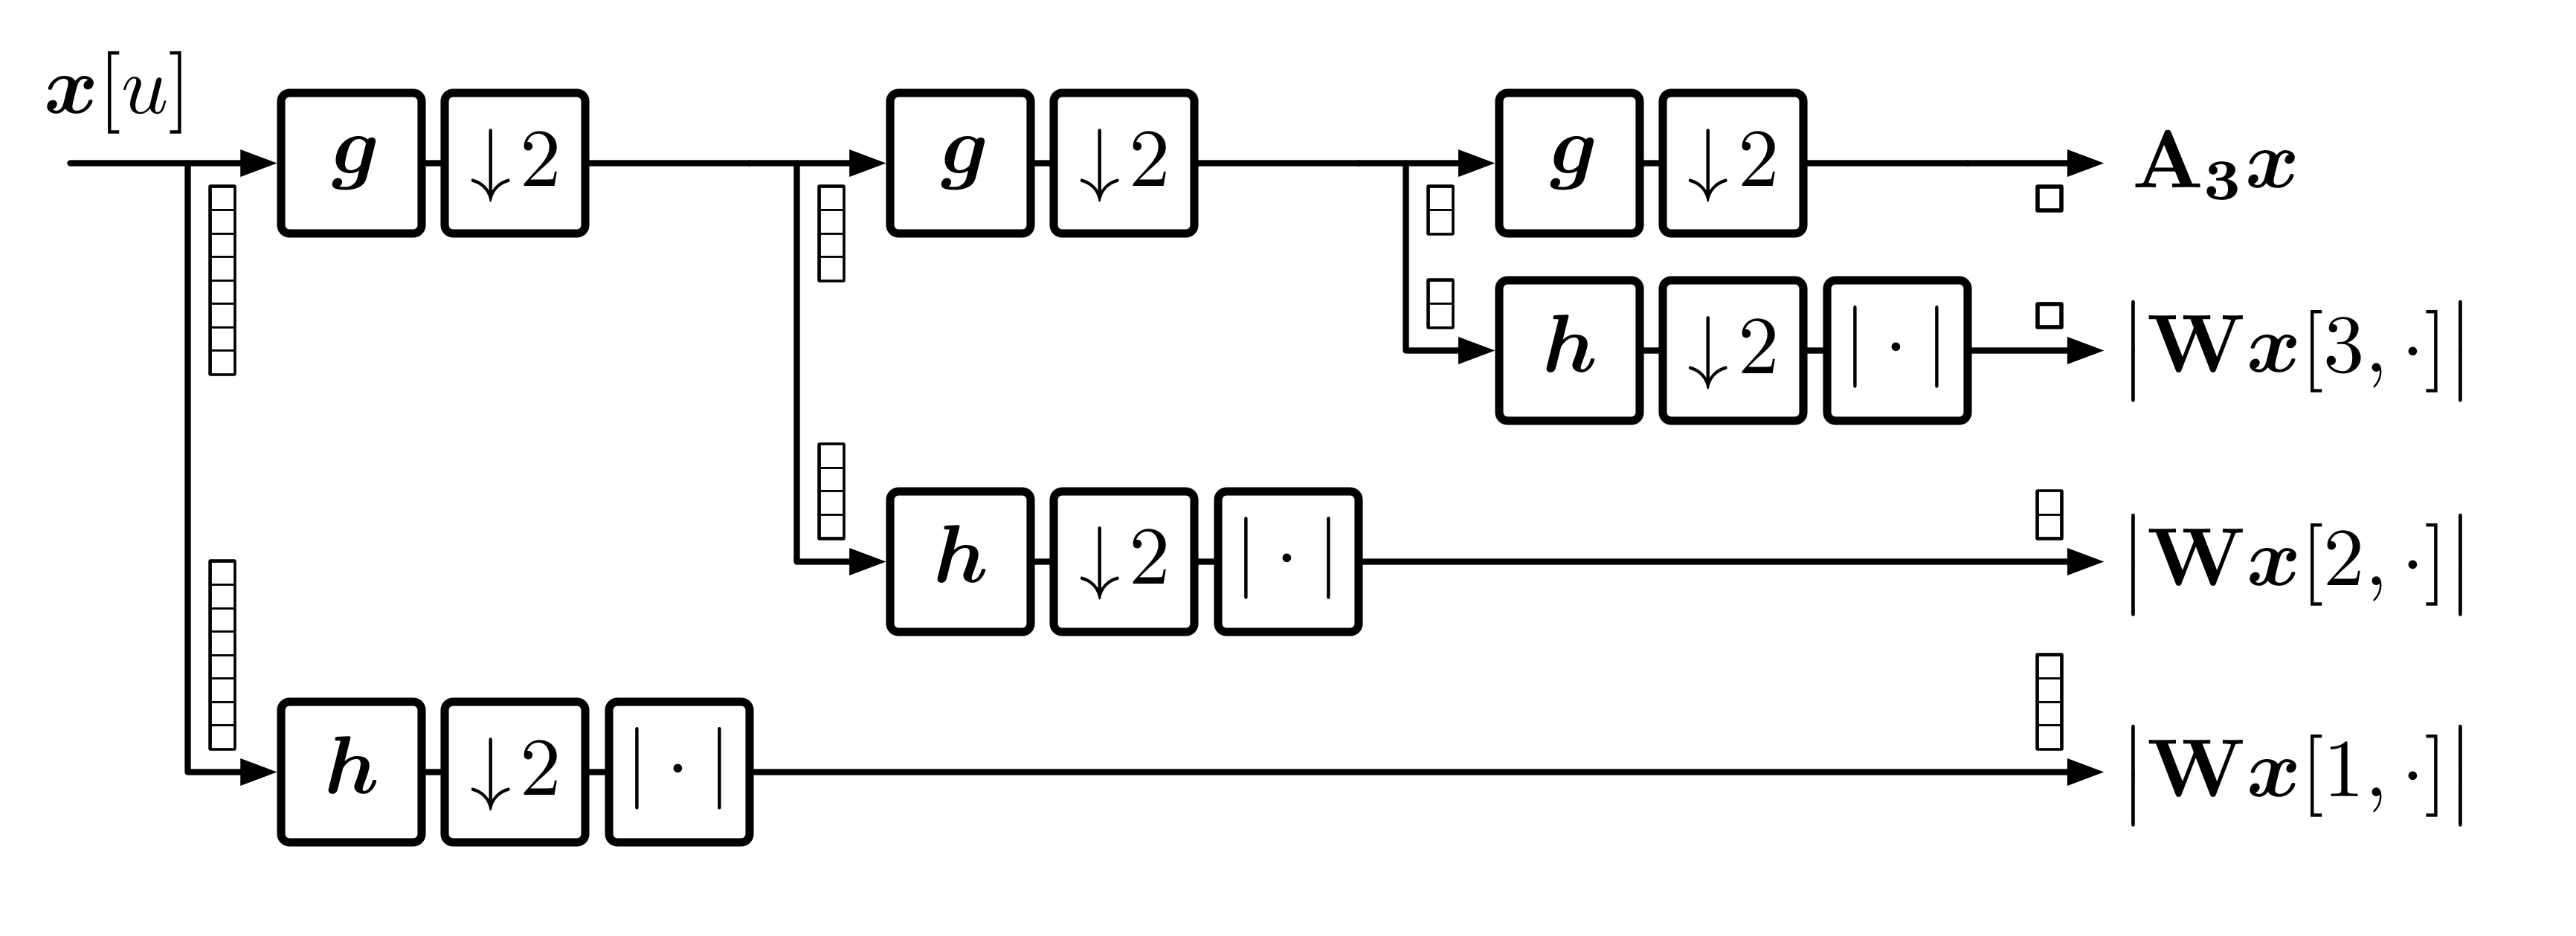
\includegraphics[width=7cm]{figs/wavelet_scheme.png}}
        \end{picture}
    \end{center}
    \protect\caption{
    Discrete wavelet transform of a signal of length 8, as implemented with a
    convolutional pyramid scheme. See text for details.
\label{fig:haar-wavelets}
}
\end{figure}

\begin{table}
	\begin{center}
	\begin{tabular}{|c|cc|}
		\hline
		& operations & memory \\
		\hline
		Matrix-vector product & $\Theta(K^2)$ & $\Theta(K)$ \\
		Fast Fourier transform & $\Theta(K (\log K)^2)$ & $\Theta(K)$ \\
		Convolutional pyramid & $\Theta(K \log K)$ & $\Theta(K)$ \\
		In-place Haar pyramid & $\Theta(K \log K)$ & $\Theta(1)$ \\
		\hline		
	\end{tabular}
	\end{center}
	\caption{
	Computational complexity and memory usage of various implementations
	of the Haar wavelet transform, for a one-dimensional signal of length $K$.
	See text for details.
	\label{table:wavelet-complexities}}
\end{table}


When applied to the chroma representation $\boldsymbol{X}(t,q,z)$, where $t$ is a temporal window, $q$ a chroma pitch class (an integer between 1 and 12), and $z$ an octave, the Haar wavelet transform encodes the sums and differences in chroma bins across octaves.
The number of output ``bands" from the Haar wavelet transform, given by $k$, determines the number of scales $J$ for which the basis Haar wavelet is dilated: $2^J = k$.

The use of the Haar wavelet transform in the feature extraction stage for our ACE system is motivated by the fact that it is stable to octave deformations -- something that the multiband representation is not. By coding for chroma relationships across varying octave scales, we are able to capture representations at both low scales (less invariance, more stability) and higher scales (higher invariance, less stability), thereby reducing the variance of the GMMs. 
	
	Upon receiving a CQT-derived pitch representation of 8 octaves $\boldsymbol{X}[t,\lambda]$, the lowest and highest octaves are thrown out of a total of 8 octaves (this follows suit from the multiband chroma representation).
$\boldsymbol{X}$ is therefore a matrix of size $T \times \Lambda$, \ie the number of frames in the song $T$ times the perceptual frequency bins $\Lambda = (12 \times 8) = 96$.
A chroma representation is then created by reshaping $\boldsymbol{X}[t, \lambda]$ into a tensor of size $T \times Q \times Z$ where $Q = 12$ (number of chroma pitch classes) and $Z = k = 8$ (number of octaves as well as number of wavelet coefficients).
In the sequel, we keep the notation $\boldsymbol{X}[t, q, z]$ for simplicity.
	
	The Haar wavelet transform is then computed iteratively over the scale $J  = log_2(k)$ and stored into a cell of size $k$, with each row in the cell containing a chroma matrix of size $T \times Q$ (same as in the multiband case, but with $k=8$ cell rows instead of 4). At each scale $j \in \llbracket1, J\rrbracket$, the chroma tensor $\boldsymbol{X}_{t,q,z}$ is reshaped to a four dimensional tensor $g$ from which the sum $g$ and difference $h$ coefficients are calculated:
	
	\begin{equation}
	\chi_{t,q,z} \rightarrow g_{t,q,w,v}
	\end{equation}
	
	where
	
	\begin{equation}
	\mathrm{size}(\chi) = (T \times Q \times Z) \hspace{1cm} \rightarrow \hspace{1cm}  \mathrm{size}(g) = (T \times Q \times 2 \times \frac{k}{2^j})
	\end{equation}
	
	$h$ takes the difference of $g$ along the third dimension ($\frac{\partial g}{\partial w} = h$). For each $v \in [1, \frac{k}{2^j}]$, the modulus $| h_{t,q,w,v}|$ is stored as a row in the output Haar wavelet representation cell. $g$ is then summed along the third dimension ($w$) and squeezed down into a three dimensional tensor (singleton dimensions due to sum removed). After iterating at all scales, the resulting $g$ is stored as the last ($k$'th) row in the output Haar cell array.
	
%%%%%%%%%%%%%%%%%%%%%%%%%%%%%%%%%%%%%%%%%%%%%%%%%%

\section{Deep Haar Scattering}\label{sec:scattering}

% don't forget to cite sifre when writing about fast deep scattering
% Explain the organization of scattering paths along the vertices of a binary cube.
Two neighboring samples $\boldsymbol{x}[2b]$ and $\boldsymbol{x}[2b+1]$ can
be retrieved, up to a permutation, from the absolute values of the subsampled QMF
decomposition $(\boldsymbol{g_{\downarrow 2}x}, \boldsymbol{h_{\downarrow 2}x})$:
\begin{equation}
\max_{u\in\{2b, 2b+1\}} \boldsymbol{x}[u] =
\dfrac{\vert \boldsymbol{g_{\downarrow 2}x}\vert [b]+
\vert \boldsymbol{h_{\downarrow 2}x}\vert [b]}{\sqrt{2}}
\end{equation}

\begin{equation}
\min_{u\in\{2b, 2b+1\}} \boldsymbol{x}[u] =
\dfrac{
\vert \boldsymbol{g_{\downarrow 2}x} \vert [b] - 
\vert \boldsymbol{h_{\downarrow 2}x} \vert [b]}{\sqrt{2}}
\end{equation}

	As opposed to the Haar wavelet transform representation, a Haar scattering representation concatenates sum and difference terms at different scales and then iterates. From the chroma representation $\chi_{t,q,z}$, we reshape to a tensor of dimension $J+2$ called $\phi$:
	
	\begin {equation}
	\chi_{t,q,z} \rightarrow \phi_{t,q,\sigma_1, \sigma_2, \ldots , \sigma_J}
	\end{equation}
	
	where the size of $\phi$ is $T \times Q \times 2_1 \times 2_2 \ldots \times 2_J$. At each scale $j \in [1, J]$, we first create a copy of $\phi$ called $\hat{\phi}$, and then concatenate the sum of $\hat{\phi}$ along scale $\sigma_j$ and the difference of $\hat{\phi}$ along $\sigma_j$, setting the result as $\phi$. We then take the modulus $| \phi | $ and iterate. 
	
\begin{figure}[t]
    \begin{center}
        \setlength{\unitlength}{1cm}
        \begin{picture}(8,7)
        \put(0.1,0){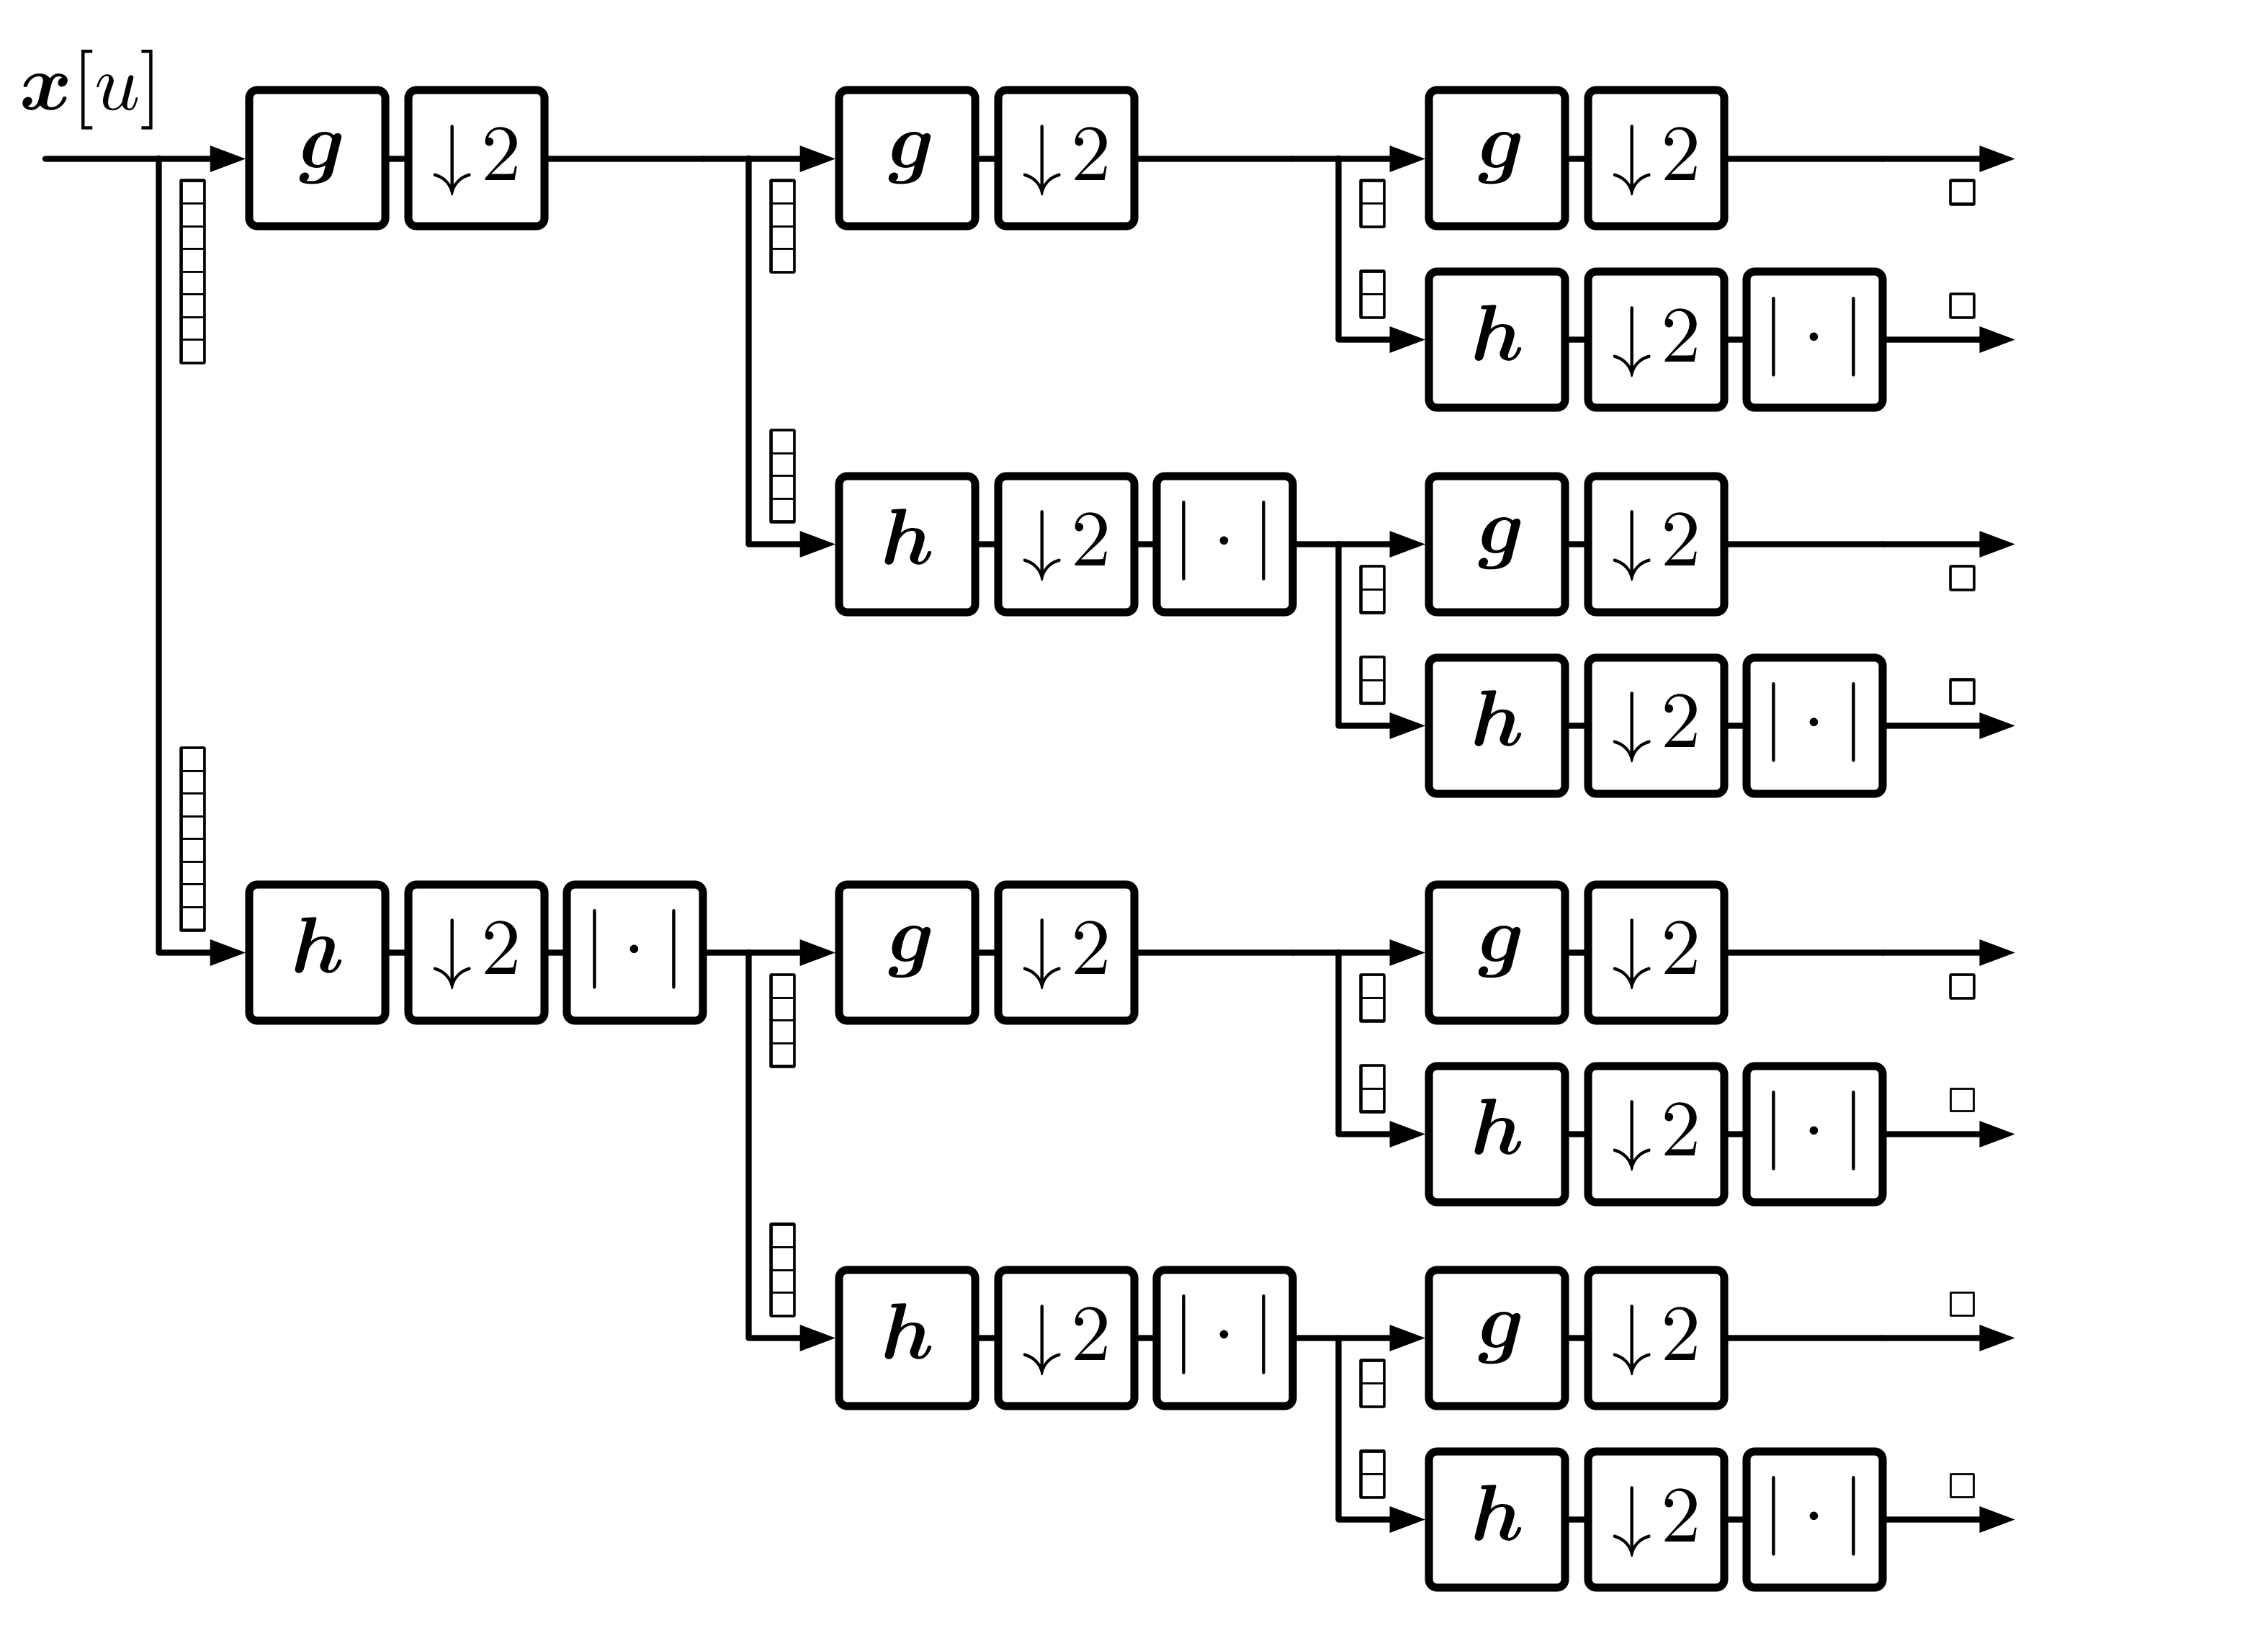
\includegraphics[width=8cm]{figs/scattering_scheme.png}}
        \end{picture}
    \end{center}
    \protect\caption{
    Deep scattering transform of a signal of length 8, as implemented with a convolutional
    pyramid scheme. See text for details.
\label{fig:haar-scattering}
}
\end{figure}

\begin{table}
	\begin{center}
	\begin{tabular}{|c|cc|}
		\hline
		& operations & memory \\
		\hline
		Matrix-vector product & $\Theta(K^3)$ & $\Theta(K^2)$ \\
		Fast Fourier transform & $\Theta(K^2 (\log K)^2)$ & $\Theta(K^2)$ \\
		Convolutional pyramid & $\Theta(K^2 \log K)$ & $\Theta(K^2)$ \\
		In-place Haar pyramid & $\Theta(K \log K)$ & $\Theta(1)$ \\
		\hline		
	\end{tabular}
	\end{center}
	\caption{Computational complexity and memory usage of various implementations
	of the deep Haar scattering transform, for a one-dimensional signal
	of length $K$. See text for details.
	\label{table:scattering-complexities}}
\end{table}
	
%%%%%%%%%%%%%%%%%%%%%%%%%%%%%%%%%%%%%%%%%%%%%%%%%%

\section{Results}\label{sec:results}

	At first, results were disappointing. As the two Haar methods operated over all octaves (i.e. number of octaves = number of coefficients), $k$ was set to 8 for these trials, and the results for the Haar wavelet representation returned a dismal 44.3 \%. Scattering performed better at 53.1 \%, but neither came close to the multiband representation.  However, when increasing the number of bands in the multiband representation from 4 to 8, accuracy for multiband plummeted to 47.6 \%. This seemed to indicate a correlation between more coefficients and decreased performance -- hinting that more stable representations needed to be used.
	
	\begin{center}
	\begin{tabular} {| c | c | c |}
	\hline
	Mode & k & \textsf{mirex} measure \\
	\hline
	Multiband & 4 & \textbf{66.8} \% \\
	& 8 & 47.6 \% \\
	
	Haar Wavelet & 4 & 55.7 \% \\
	 & 8 & 44.3 \% \\
	 
	 Haar Scattering & 4 & 60.2 \% \\
	  & 8 & 53.1 \% \\
	\hline
	\end{tabular}
	\end{center}
	
	To decrease the number of coefficients in the wavelet representations from $k=8$ down to $k=4$, neighboring octaves were averaged together, and the wavelet coefficients were the constructed over a scale of $J = log_2(k) = 2$. Both Haar wavelet methods benefit from this decrease of scale, as the Haar Wavelet accuracy jumps up to 55.7 \% accuracy (an increase of 11.4\%) and the Haar Scattering accuracy becomes 60.2 \% (an increase of 7.1 \%). While still not quite as good as the multiband representation, Haar scattering begins to come a bit closer.
	
%%%%%%%%%%%%%%%%%%%%%%%%%%%%%%%%%%%%%%%%%%%%%%%%%%

\section{Discussion}\label{sec:discussion}

Haar wavelet analysis does not lead to terrible results, but nor does it achieve the same level of accuracy as the typical multiband chroma approach. Why? One reason is that the wavelet coefficients, both in the Haar wavelet transform and the deep Haar wavelet scattering methods, lack local context. This is done primarily to achieve octave invariance and to stabilize the chord recognition system to deformations, but the Haar representations seem to go too far by completely delocalizing along pitch. 
	
	Higher harmonics have significantly different behavior than lower ones. While in lower octaves the fundamental frequencies stand out, at higher octaves the harmonics start to clutter the chroma space at low amplitudes, making detection of the fundamental at upper harmonics very difficult. The multiband chroma representation creates, at every frame, $k$ chroma representations which then vote on a chord using GMMs. Chroma vectors at high octaves are likely poorer voters than those at lower octaves, where fundamentals are more strongly represented. The Haar representations delocalize information completely along pitch, blurring the more useful information at lower octaves with the less useful information at higher octaves -- resulting in less accurate voting. 

%%%%%%%%%%%%%%%%%%%%%%%%%%%%%%%%%%%%%%%%%%%%%%%%%%

% For bibtex users:
\bibliography{WaveletScatteringISMIR2016}

% For non bibtex users:
%\begin{thebibliography}{citations}
%
%\bibitem {Author:00}
%E. Author.
%``The Title of the Conference Paper,''
%{\it Proceedings of the International Symposium
%on Music Information Retrieval}, pp.~000--111, 2000.
%
%\bibitem{Someone:10}
%A. Someone, B. Someone, and C. Someone.
%``The Title of the Journal Paper,''
%{\it Journal of New Music Research},
%Vol.~A, No.~B, pp.~111--222, 2010.
%
%\bibitem{Someone:04} X. Someone and Y. Someone. {\it Title of the Book},
%    Editorial Acme, Porto, 2012.
%
%\end{thebibliography}

\end{document}
